\chapter{Resultados Alcançados}\label{cap:result}

Para validar a comunicação foram idealizados dois ensaios: o primeiro com o objetivo de testar o fluxo completo de troca de dados entre um nó ROS e uma aplicação embarcada no FPGA; o segundo ensaio teve o objetivo de testar um fluxo grande de dados trafegando entre o ROS e o SoC.

O objetivo do primeiro ensaio era verificar a comunicação completa entre o nó ROS e um IP sendo executado no FPGA. Para isso,  foi projetado um circuito simples que calcula o dobro de um número,  este circuito foi instanciado no FPGA, a \textit{HPS-to-FPGA Lightweight} bridge foi utilizada para realizar a comunicação entre o servidor, rodando no HPS, e o FPGA. No nó cliente, rodando no ROS, foram configurados dois tópicos, um para o número a ser enviado e outro para receber o resultado calculado pelo FPGA, da mesma maneira que mostra o esquema da Figura \ref{fig:arquitetura}. A comunicação foi estabelecida e o sistema se comportou como esperado.

O segundo ensaio tinha a intenção de testar a sobrecarga de dados na rede e avaliar o comportamento da mesma. Neste teste foi realizado o envio de uma \textit{stream} de vídeo com resolução de 1280x720 em 15 fps capturada a partir de uma webcam dentro do ambiente ROS, ou seja, um nó ROS acessa a webcam e disponibiliza a \textit{stream} de vídeo em um tópico sendo publicado e uma frequência de 15Hz. A partir deste ensaio foi possível realizar a estimativa de largura de banda utilizada e o \textit{delay} gerado na comunicação. No gráfico da Figura~\ref{fig:speed} podemos ver a velocidade da comunicação, em bits por segundo, em função do tempo de transmissão. As velocidades alcançadas superaram a barreira dos 400 Mbps.

\begin{figure}[ht]
	\caption{Gráfico velocidade de transmissão}
	\begin{center}
		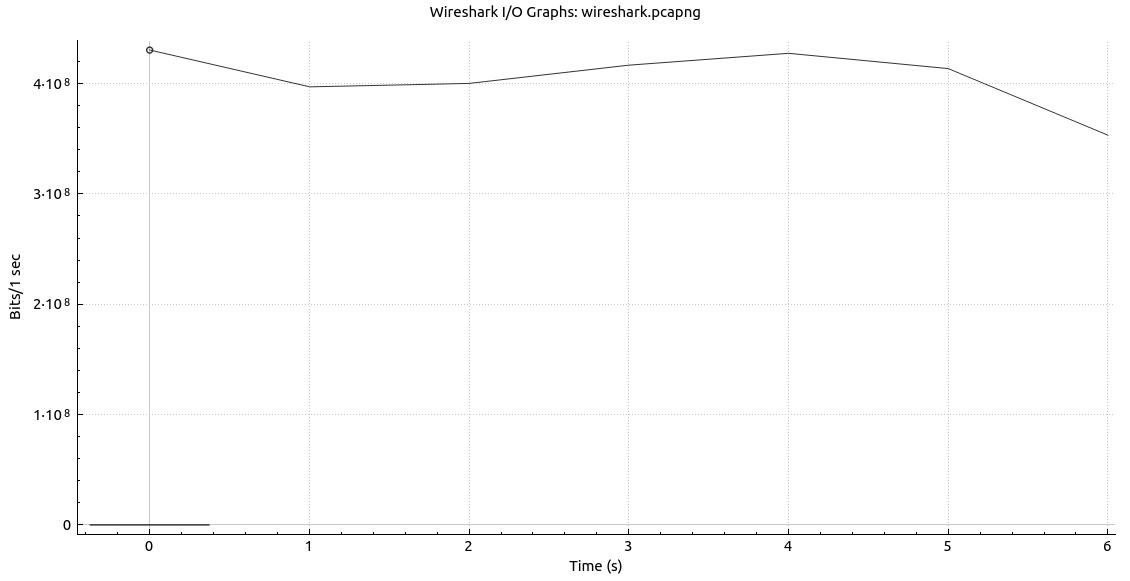
\includegraphics[scale=0.42]{imagens/speed.jpg}\\
		{\small \textbf{Fonte:} Elaborado pelo autor}
    \end{center}\label{fig:speed}
\end{figure}

Os atrasos gerados podem ser vistos na Figura~\ref{fig:delay}, onde é possível observar o \textit{Round Trip Time} (RTT), que é o atraso total de um pacote TCP, ou seja, o tempo que um pacote leva para ir da origem ao destino e retornar à origem. Os atrasos máximos ficaram por volta de 10ms. 

\begin{figure}[ht]
	\caption{Atrasos gerados durante a comunicação}
	\begin{center}
		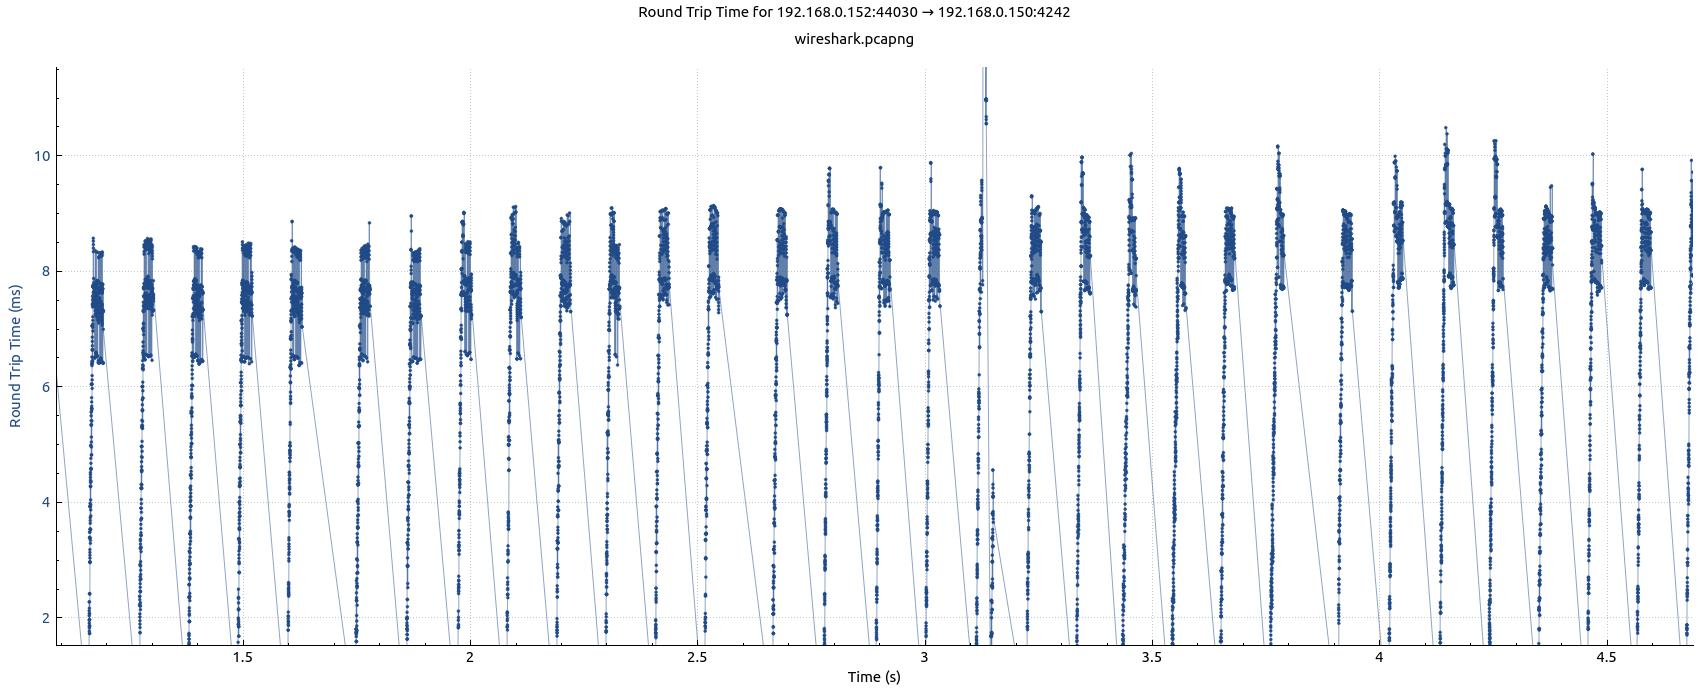
\includegraphics[scale=0.35]{imagens/delay.jpg}\\
		{\small \textbf{Fonte:} Elaborado pelo autor}
    \end{center}\label{fig:delay}
\end{figure}

